%!TEX root = these.tex

\chapter[Analyse de l'acquisition de cibles mobiles]{Analyse de l'acquisition de cibles mobiles}
\minitoc
\label{chap4}
\cleardoublepage

\section{Introduction}
	Dans ce chapitre nous présentons les résultats d'une étude empirique visant à caractériser les performances de sélection de cibles mobiles en fonction de la nature de leurs mouvements, dans un contexte aussi simple que possible : un ordinateur de bureau avec un écran monoscopique et une souris. Notre objectif étant de mieux comprendre cette tâche, dans le but éventuel d'aboutir à un modèle fiable, nous avons en effet cherché à limiter autant que possible l'influence de facteurs tels que la stéréoscopie (éventuellement adaptative), la nécessité de déplacements du corps entier, l'utilisation de périphériques peu familiers, etc. 
	
	Nous revenons premièrement sur le modèle de génération de mouvement introduit dans le chapitre~\ref{chap3}, ses capacités et limitations, et son extension 3D. Nous proposons d'autres extensions de ce modèle permettant de gérer les cas actuellement hors de sa portée.
	
	Nous étudions ensuite l'effet individuel des paramètres d'angle, de fréquence et de vitesse issus de notre modèle, puis les interactions entre ces effets. Nous relions ces paramètres et les conditions qu'ils engendrent aux impressions subjectives des participants à notre étude, afin d'établir quels facteurs perceptifs ou cognitifs influent sur les performances de sélection, selon la nature du mouvement des cibles.

	Dans ce but, nous examinons d'une part les profils de vitesse du curseur lors des tâches de sélection, en mesurant la durée relative de la phase balistique, et d'autre part le pouvoir prédictif des enveloppes convexes, introduites dans le chapitre~\ref{chap3}.
	
	Sur la base des enseignements que nous en tirons, nous proposons un guide pour la conception de techniques de sélection spécifiquement orientées vers les cibles mobiles, en précisant comment la nature des mouvements influe sur les contraintes imposées par la tâche, et sur les solutions possibles.

\section{Génération de mouvements}
	Si notre objectif est de caractériser les performances de sélection pour des cibles mobiles en fonction de la nature de leurs mouvements, notre intérêt se porte plus particulièrement sur les cibles de mouvements \og erratiques \fg{}, \og imprévisibles \fg{}, ou rappelant ceux d'une mouche.
	
	Ce focus a principalement deux motifs : premièrement, les chercheurs spécialisés dans la biologie structurale tentant d'utiliser des techniques de simulation de dynamique moléculaire interactive (voir le chapitre~\ref{chap1}) nous ont exprimé leurs difficultés d'interaction avec leurs systèmes, et particulièrement de sélection. Deuxièmement, de rapides tests empiriques suggéraient que les mouvements de ce type causaient les plus grandes difficultés pour des tâches de sélection.
	
	\subsection{Modèle VFA}
	Afin de tester cette hypothèse, nous avons conçu un modèle de génération de mouvements permettant, à l'aide d'un nombre de paramètres aussi petit que possible, de générer des mouvements aussi variés que possible dans leur nature. Pour rappel, il s'agit du modèle évoqué dans le chapitre~\ref{chap3}, et décrit par les paramètres suivants, pour définir le mouvement d'un objet de vecteur direction $\vec{dir}$ :
	
    \begin{enumerate}
    	\item La vitesse $V$ à laquelle l'objet se déplace ;
    	\item La fréquence $F$ des changements de $\vec{dir}$ ;
    	\item L'angle maximal $A$ de ces changements de direction : à chaque période $T = \frac{1}{F}$, $\vec{dir}$ subit une rotation d'un angle $\alpha$ échantillonné uniformément dans l'intervalle $[-A, +A]$.
    \end{enumerate}
    
    Du fait de son fondement sur les paramètres $V$, $F$ et $A$, nous appellerons simplement ce modèle $VFA$.
    
    \subsection{VFA en 3D}
    Quelques observations s'imposent. Tout d'abord, bien que décrit ici pour deux dimensions, ce modèle est naturellement extensible à l'espace tridimensionnel. En effet, les paramètres $V$, $F$ et $A$ ne changent pas ; seule un ajustement est nécessaire : la rotation du vecteur direction de l'objet animé doit se faire selon un axe qui, pour que la rotation effective soit toujours la même pour un angle donné, doit être orthogonal à $\vec{dir}$. Notre modèle étendu VFA3D fonctionne donc comme le modèle VFA, mais avec un axe de rotation orthogonal à $\vec{dir}$ choisi aléatoirement.
    
    \subsection{Un modèle puissant mais limité}
	Les capacités offertes par le modèle VFA sont très nombreuses, mais demeurent limitées, et ne peuvent couvrir tous les besoins possible en matière de génération de mouvement aléatoire.
    
    \subsubsection{Vitesse constante}
    Comme nous l'avons partiellement montré dans le chapitre~\ref{chap3}, le fait de varier les paramètres, en particulier $F$ et $A$, permet de générer des types de mouvement subjectivement très différents (voir les figures~\ref{fig:motion1530}, \ref{fig:motion4560}, \ref{fig:motion7590}, \ref{fig:motion105120}, \ref{fig:motion135150} et \ref{fig:motion165180}), et d'enveloppes convexes de tailles très différentes également (voir la figure~\ref{fig:trajAreas}). Néanmoins, et outre le problème des objets autocorrélés, notre modèle repose notamment sur une vitesse constante, ce qui, de fait, exclut tous les objets susceptibles d'accélérer. Là encore, ce choix fut fait pour limiter le nombre de paramètres, toujours dans l'objectif d'atteindre un compromis entre la simplicité du modèle et sa capacité à générer des mouvements que nos sujets puissent percevoir comme fondamentalement différents.
    
	Nous souhaitions tout particulièrement pouvoir générer du mouvement perçu comme \og régulier \fg{} ou \og prévisible \fg{} ainsi que du mouvement \og irrégulier \fg{}, \og saccadé \fg{} ou \og imprévisible \fg{}.
    
   	\subsubsection{Pas de véritable autocorrélation}
	Une autre obsevation très importante est que ce modèle ne peut générer que du mouvement markovien. En effet, à l'instant $t+1$, la rotation de $\vec{dir}$ générée est totalement indépendante de celle éventuellement générée à $t$, ou plus généralement de la dernière rotation générée, si elle existe. Cela ne signifie pas que $\vec{dir}_{t+1}$ soit indépendant de $\vec{dir}_{t}$, et il ne l'est pas, mais que le changement de direction à tout instant est indépendant du passé de l'objet concerné.
    
    Il en résulte que ce modèle ne peut générer du mouvement permettant d'étudier les performances de sélection sur des objets autocorrélés, tels que nous les avons définis et énumérés au cours du chapitre~\ref{chap3}. Ce choix reflète d'une part notre focus originel sur les simulations moléculaires (où il y a une demande claire émanant des utilisateurs) et d'autre part une volonté de conserver un modèle aussi simple que possible, afin de le rendre plus facile à utiliser, mais aussi pour pouvoir évaluer un échantillon représentatif des types de mouvements qu'il peut générer dans un laps de temps raisonnable pour une étude empirique, compte tenu notamment de la fatigue des sujets.
    
    \subsubsection{Mouvements pseudo-autocorrélés}
	Remarquons tout de même qu'une trajectoire générée par notre modèle peut, au moins temporairement, approximer un mouvement autocorrélé. Attendu qu'une tâche de sélection, pour peu qu'elle ne soit pas trop difficile, peut se dérouler sur une durée inférieure ou égale à la durée pendant laquelle le modèle VFA peut approximer un mouvement autocorrélé, il n'est pas nécessairement inutile pour étudier les performances de sélection de ces objets. On privilégiera dans ce cas de très fortes valeurs de $F$ et de très faibles valeurs de $A$. La figure~\ref{fig:autocorr} fournit deux exemples de telles trajectoires que nous proposons d'appeler pseudo-autocorrélées, générées avec $F \in \{30,120\}$ et $A \in \{1,2\}$.
	
	\begin{figure}[!htb]
		%\centering
		\begin{subfigure}[t]{0.49\textwidth}
			\centering
			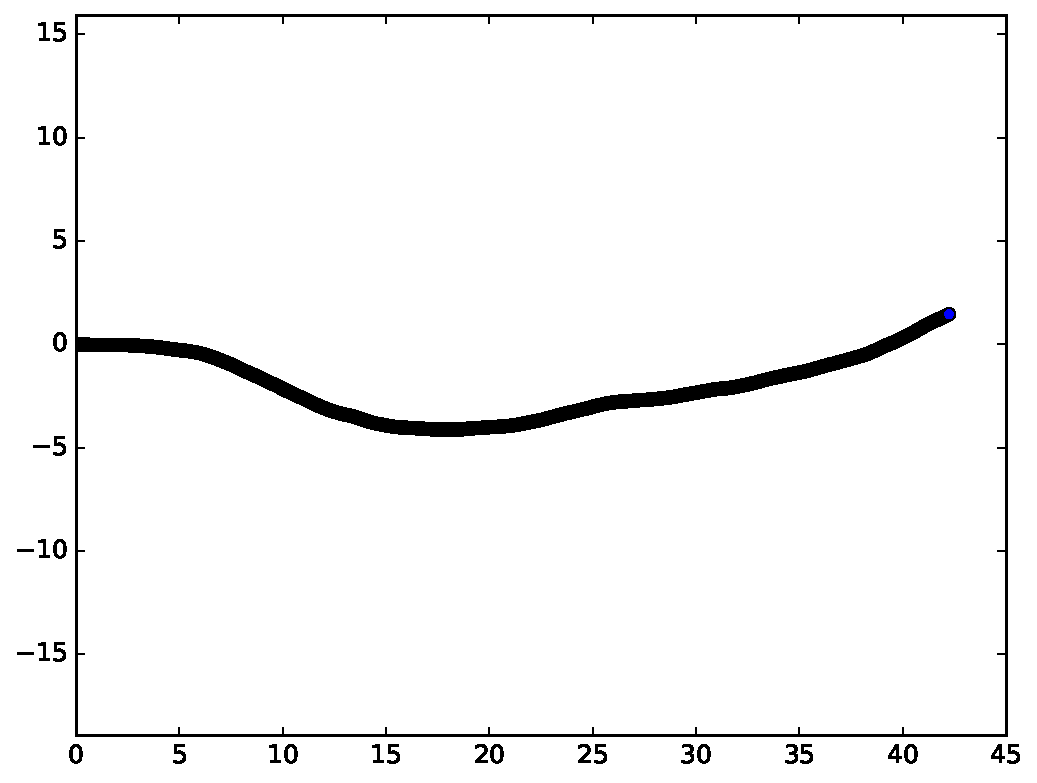
\includegraphics[width=\textwidth]{figures/ch4/ac_2_19_1_120a}
			\caption[Mouvement pseudo-autocorrélé A]{$F = 120$ et $A = 1$.}
			\label{fig:ac1_120A}
		\end{subfigure}
		~
		\begin{subfigure}[t]{0.49\textwidth}
			\centering
			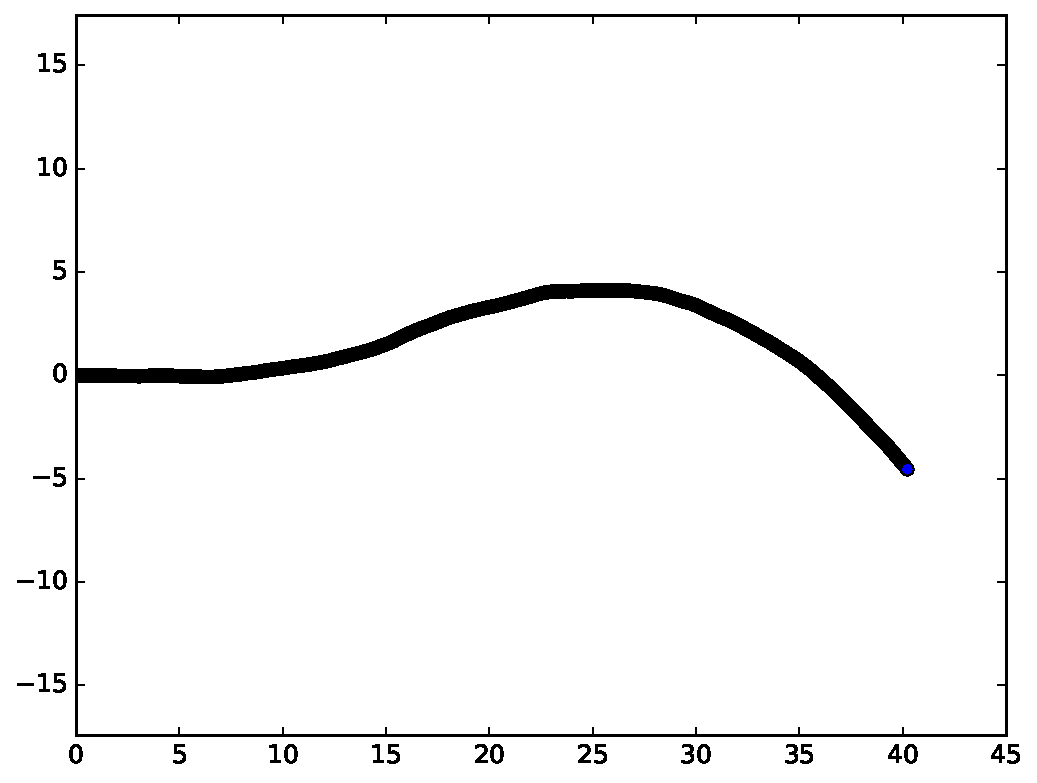
\includegraphics[width=\textwidth]{figures/ch4/ac_2_19_1_120b}
			\caption[Mouvement pseudo-autocorrélé B]{$F = 120$ et $A = 1$, bis.}
			\label{fig:ac_1_120B}
		\end{subfigure}
		~
		\begin{subfigure}[t]{0.49\textwidth}
			\centering
			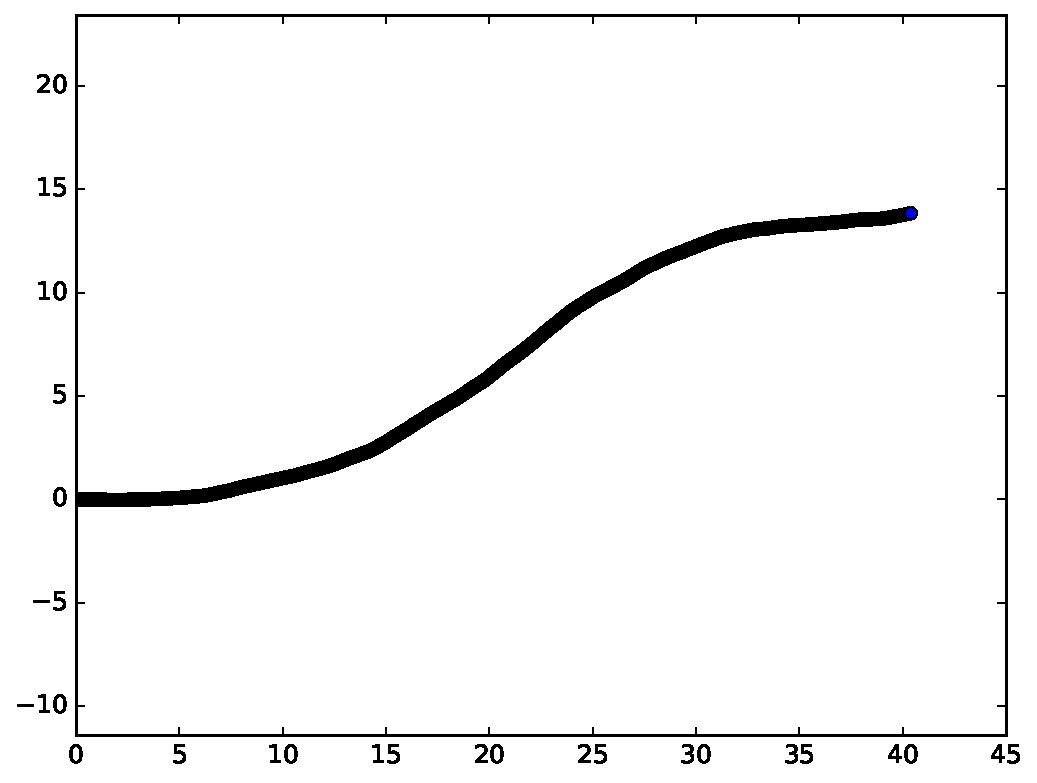
\includegraphics[width=\textwidth]{figures/ch4/ac_2_19_2_30}
			\caption[Mouvement pseudo-autocorrélé B]{$F = 30$ et $A = 2$.}
			\label{fig:ac_2_30}
		\end{subfigure}		
		~
		\begin{subfigure}[t]{0.49\textwidth}
			\centering
			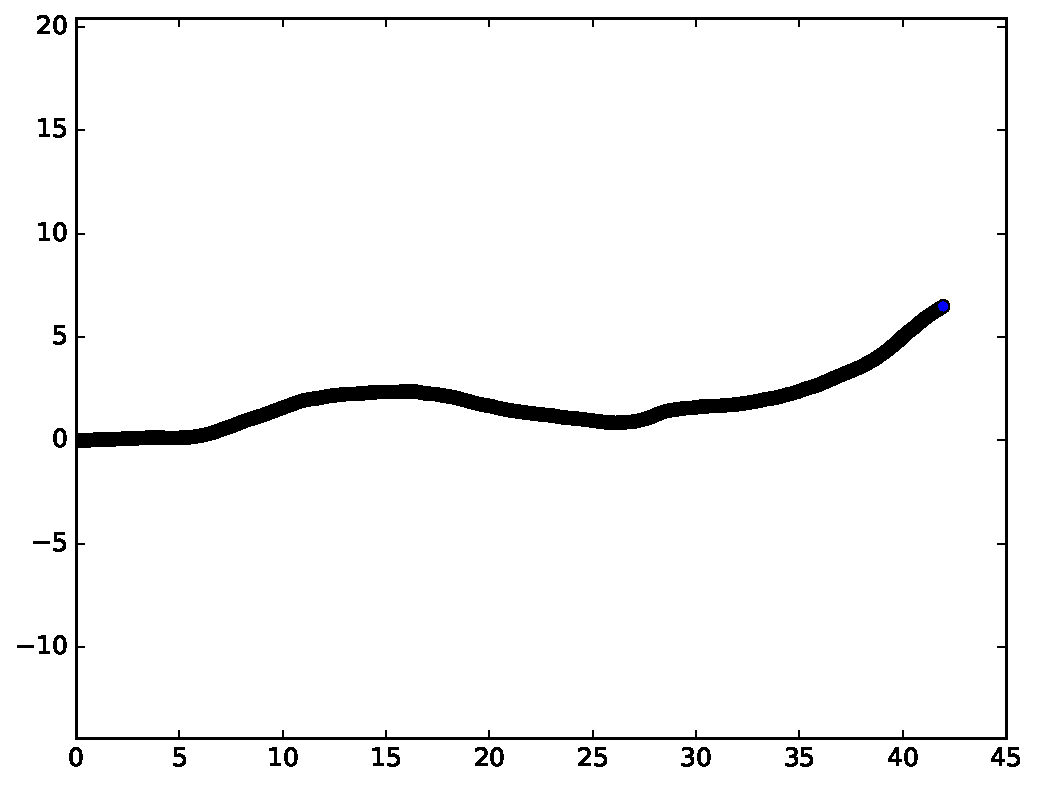
\includegraphics[width=\textwidth]{figures/ch4/ac_2_19_2_60}
			\caption[Mouvement pseudo-autocorrélé B]{$F = 120$ et $A = 1$, ter.}
			\label{fig:ac_1_120C}
		\end{subfigure}
		\caption{Trois trajectoires générées avec les mêmes valeurs $F = 120$~Hz et $A = 1\degree$, et une avec $F = 30$~Hz et $A = 2\degree$. Dans tous les cas, $V = 2,19$~cm/s. Ces trajectoires ressemblent à celles que l'on pourrait attendre d'objets autocorrélés, tels que des véhicules, par exemple.}
		\label{fig:autocorr}
	\end{figure}
    
    \subsection{Proposition de modèles de génération de mouvements autocorrélés}
    Les objets autocorrélés présentent néanmoins un intérêt certain, et les trajectoires pseudo-autocorrélées ne sont que des approximations qui peuvent s'avérer unsuffisantes. Ces objets pourraient faire l'objet d'études spécifiques pour lequelles de telles approximations ne seraient pas suffisantes. Nous proposons donc ici deux modèles différents permettant de générer des mouvements réellement autocorrélés.
    
    \subsubsection{Modèle VFA à mémoire}
    Une première option pour un modèle adapté aux objets autocorrélés serait d'adapter le modèle VFA en lui ajoutant une mémoire, par exemple une mémoire du dernier changement de direction de l'objet concerné. L'on retiendrait ainsi l'angle du changement de direction à l'instant précédent ($\alpha_{t-T}$, avec $T = \frac{1}{F}$), et l'on pourrait appliquer un nouveau changement avec un angle plus ou moins proche de ce dernier, selon des paramètres. L'équation~\ref{eq:vfamem} présente une possibilité, où $\alpha$ est échantilloné entre $-A$ et $+A$, et $c_{ac} \in [0,1]$ est un coefficient d'autocorrélation.
    
    \begin{equation}
		\alpha_{t} = \alpha_{t-T} \times c_{ac} + \alpha (1 - c_{ac})
		\label{eq:vfamem}
    \end{equation}
    
	Ainsi, lorsque le coefficient d'autocorrélation est nul, le système devient markovien ; lorsqu'il vaut 1, $\alpha_{nT}$ est constant (avec $n \in \mathbb{N}$). De fait, s'il est non nul, l'objet aura un mouvement circulaire s'il est ciné-continu et régulier s'il est ciné-discret , s'il est nul, le mouvement sera rectiligne dans les deux cas.
    
    \subsubsection{Modèle newtonien}
    Une seconde option ayant le mérite d'avoir un certain sens physique consisterait à considérer chaque objet comme une particule dotée d'une masse, et de la soumettre à une force qui, elle, serait régie par un modèle de type VFA, éventuellement modifié pour remplacer la vitesse par la norme de la force, notamment. Sans doute serait-il également opportun d'appliquer une force de friction afin d'éviter que l'application (même approximativement) constante d'une force (et donc d'une accélération\footnotemark{}) ne mène à des vitesses potentiellement croissantes et non bornées.
    
    \footnotetext{Rappelons que, d'après la seconde loi de Newton~\cite{newton1833philosophiae}, $\vec{F} = m\vec{a}$ où $F$ est une force, $m$ est la masse de l'objet sur lequel elle agit, et $\vec{a}$ est l'accélération de l'objet, soit $\vec{a} = \frac{\vec{F}}{m}$, où l'on voit bien que l'application d'une force constante à un objet de masse constante mène à une accélération constante, donc à une vitesse croissant linéairement. En l'absence de résistance à $\vec{F}$, la vitesse n'est pas bornée.}
    
    Le modèle nécessiterait un calibrage précis pour obtenir le comportement souhaité, notamment en ce qui concerne les masses des objets ou le coefficient de friction. Notons par ailleurs que, sauf dans certains cas particuliers (et après une période dynamique) les vitesses des objets ne seraient pas constantes pour une norme de $\vec{F}$ donnée, ce qui distinguerait ce modèle newtonien du nôtre (VFA). En soi, ce n'est pas nécessairement un problème --- et peut même être un avantage --- mais cela complique le contrôle des propriétés d'un environnement synthétique créé pour mener une étude empirique.

\section{Expérience et protocole}
We conducted an experiment with 13 right-handed participants, aged 14 to 56. They were asked to click with a mouse on a moving target displayed on a desktop monitor.

	\subsection{Dispositif expérimental}
	The input device was a standard mouse without acceleration, moving a
standard crosshair pointer on a Dell UltraSharp U2412M 24” display. The task was
performed in a square window of 1000 pixels (about 23.87cm).

	\subsection{Task and Conditions}
	The task consisted in selecting one circular target among 50,
with a fixed diameter of 5.4mm. The 49 “distractors” were displayed in gray, and the
target to select in red (see Figure 3(b)). Both the target and the distractors moved
according to the current condition, defined by the S, F and A parameters, and bounced
off the edges of the window. To control the pointing amplitude, the motion of the
distractors was constrained so that after selecting a target, the distance between the
mouse cursor and the next target was constant (of about 7.96cm). When the participant successfully selected the red target, it briefly turned green while the next target to
select turned red at the same time.
Selection involves a trade-off between speed and accuracy [4], and users can adopt
different approaches to this trade-off. In order to minimize such variation in selection
strategy, participants were instructed to select the target as fast as possible but with at
most 5 attempts. The number of remaining attempts for each trial was displayed in the
top left corner of the window. After the last try, the word “failure” was displayed and
the participant was asked to keep trying to select the target, but without trying to
minimize errors. Thus, failures are not absolute, but indicate critical conditions for
which selection is very difficult.
We tested all combinations of the following (S,A,F) values, replicated 4 times:
 S: 0.73, 1.46 and 2.19 cm/s (3 values);
 F: 1, 2, 4, 8, 13, 20 and 30Hz (7 values);
 A: 0, 30, 60, 90, 120 and 180 degrees of arc (6 values).
An additional baseline condition was added with static targets, which was replicated 20 times. When A = 0, targets move in straight lines. In summary, we tested a total of 3×6×7 + 1 = 127 conditions, and 524 trials (126×4 + 1×20) per participant.

\subsection{Procédure et collecte de données}
Each session lasted approximately 40 minutes, including a training phase of over 50 trials, after which participants felt comfortable
with the task. Short breaks were allowed after 25\%{}, 50\%{} and 75\%{} of the trials were
completed. At the end of the session, participants were administered a short question-
naire about their perception of the different classes of motion and the strategies they
had adopted.
We collected Selection Time from the moment the target turned red to the success-
ful click, Erroneous Clicks (i.e. clicks outside of the target disk), and Failures (i.e.
last erroneous clicks of the 5 tries).

\section{Résultats : performances de sélection}
	All the values presented here are averaged across the subjects. Performance in the
easiest conditions was relatively stable across participants: our slowest participant
was less than 4 times slower than the fastest one for straight motion. However, there
was a considerable amount of variation for the most difficult conditions (by a factor
of over 18 from the fastest to the slowest participant). We therefore normalized selec-
tion times to avoid bias from the slowest participants: for each participant, the result-
ing averages of normalized selection times (ANSTs) are the average of selection time
per condition, normalized according to the most difficult condition for the given par-
ticipant. Therefore, if a condition has an ANST of 0.75 for a given participant, it
means that this participant needed 75\%{} as much time on average to select targets in
this condition as in the condition he/she found most difficult. Because the condition
that was precisely the most difficult may be slightly different for each participant, no
condition has an average ANST of 1.0 across all subjects.
The number of errors ranges from 0 to 5. An error rate of 3.5 for a given condition
means that on average, participants made 3.5 failed clicks for each trial in that condi-
tion. A failure rate of 50\%{} for a given condition means that on average, 50\%{} of the
trials in that condition were failed, i.e. that participants made at least 5 failed clicks in
50\%{} of their trials. Note that because of growing concerns in various research fields
over the limits of null hypothesis significance testing for reporting and interpreting
experimental results [1, 2], our discussions are based on effect sizes (reported as per-
cent differences1).

	\subsection{Vitesse}
	We observed that both selection time and error rate increase when speed in-
creases, as illustrated in Figure 1(a): average ANST at the highest speed (37\%{}) is
higher than in the lowest one (17\%{}) with a percent difference of 74\%{}. We observe
that selection time and error rates are roughly affine functions of speed. We only in-
cluded the plots for A = 90, but the results for all other values of A are very similar.

	\subsection{Angle}
	Parameter A exhibits more complicated tendencies, with an interaction with
both S and F. At low speed, A has a small effect on selection times (for S = 0.73 and
F = 4, when A = 0, ANST = 14\%{} and when A = 120, ANST = 20\%{}; percent differ-
ence of 33\%{}, the highest observed at this speed) but a bigger effect at high speed (for
S = 2.19, at the same A and F, ANSTs are respectively 21\%{} and 54\%{}; percent differ-
ence of 90\%{}). A possible explanation is that at low speed, selection is almost as easy
as with static targets, regardless of the nature of the motion. Figure 1(c) illustrates the
effect of A at high speed. We observe that as long as frequency is low, higher values
of A imply higher selection times. However, as F increases, the effect of A on selec-
tion time is changed: after steadily increasing with A, selection time reaches a plateau,
and then decreases. Furthermore, the value of A associated with this plateau (Apeak)
depends on F: as F increases, Apeak decreases.
We also observed that the number of errors and failure rates follow the same trends
and that at medium speed, these trends are similar but less pronounced.

	\subsection{Fréquence}
	A similar pattern can be observed for frequency: F has a smaller effect on
selection time when speed is low, but a larger one at high speed. On Figure 1(d), we
observe that for lower values of A, higher frequencies are correlated with higher se-
lection time, but for higher values of A, the trend changes. When A is high, selection
time increases with F up to a certain peak (Fpeak) and then decreases. Furthermore, the
value of Fpeak decreases as A increases. Trends for number of errors and failure rates
are consistent with those observed for selection time, and as for angle widths, trends
at medium speed are similar to those at high speed, although less pronounced.

\section{Analyse exploratoire}
	We also considered our parameter space as a whole in order to identify general trends.
The heat maps in figures 2(a) and 2(b) represent the ANSTs for medium and high
speeds. In each of those heat maps, A stands on the horizontal axis, and F on the ver-
tical one. Each intersection is thus the average of ANSTs for the corresponding condi-
tion. The heat maps in figures 2(b), 2(c) and 2(d) present the highest speed we tested,
since it resulted in the most pronounced effects of A and F. In Figure 2(b), we observe
that a region of the heat map approximately centred on the main diagonal (from top-
left to bottom-right) exhibits the highest selection times. Figure 2(c) displays the av-
erage error rates for each condition, which are correlated with selection times. Finally,
failure rates are presented in figure 2(d).
These heat maps suggest that selection is especially difficult for combinations of
wide angles with low frequencies, narrow angles with high frequencies, or medium
angles with moderate frequencies.
Figure 2 - Selection performance as a function of A and F, for different values of S.

	\subsection{Prévisibilité selon les angles et fréquences}
	The trends highlighted above suggest that the product A×F (angle width by frequency) might roughly predict selection performance for erratic targets. We plotted this product against selection time in figure3(a), and it reveals that an index of difficulty (or predictability) for irregular motion could be derived from A×F. Furthermore, when A×F reaches a certain value AFpeak,
which in our data is around 1,100, selection time is maximal. We suppose that AFpeak
would vary in different conditions, e.g. target width or pointing distance as described
by Fitts’ law, but it remains stable for the three different speeds we have tested, and
therefore probably independent of this parameter. As mentioned before, we observed
error rate to be generally strongly correlated with selection time, and so to also de-
pend on the A×F product.

	\subsection{Impressions subjectives}
	The answers to our questionnaire were consistent with, and complementary to, our quantitative results. Indeed, 92\%{} of our participants were able to identify different categories of motion: 77\%{} of them identified at least three major categories, together with two or three corresponding selection strategies.
Figure 3 - Selection time as a function of A×F. Screenshot of the application.

	\subsection{Catégories et stratégies}
	Participants first described rather steady motion, in roughly straight lines, with few or small deviations. In the second case, they identified “jerky” or “erratic” motion that they characterized by frequent, significant changes in direction. In the third case, they described the motion as “Brownian”, or “oscillations” or “vibrations”. More interestingly, 92\%{} of them explained that they would try to anticipate the target’s movement and to intercept it, and those who had identified a steady category specifically linked this strategy to it. However, our participants had no “clever” way of catching jerky targets, and would simply try to be fast enough and click a lot, thus making many errors. For the vibrating category, 69\%{} of them said
they would aim for the “average” position of the target over a short period of time, and either try to intercept it or just click and hope for the best.

	\subsection{Interprétation}
	The steady category reflects how our participants perceived the con-
ditions where both angle width and change frequency were low. The jerky category
relates to the difficult diagonal of our heat maps, and the vibrating category is the one
with both high frequency and angle width. The important observation is that the strat-
egy of anticipation requires a certain degree of predictability, since one can only an-
ticipate what one can predict. Likewise, aiming for the average position of a target is a
prediction. On the other hand, the jerky category seems to be very difficult to predict.
We therefore conclude that the steady and vibrating categories of moving targets
are relatively easy to acquire because their movements are quite predictable, whereas
jerky targets are more difficult because less predictable. Of course, the borders be-
tween these categories are hard to determine formally and are likely to depend on the
user perception of the movement.

\section{Conclusion and perspectives}
We have proposed a way to characterize the erratic behavior of moving targets with
three parameters: speed, angle width and frequency, and tested pointing performance
when varying these parameters. We have shown that the nature of target motion af-
fects pointing performance, which is not captured by Fitts’ law’s index of difficulty.
The latter can only describe the best case, and does not indicate that acquiring fast,
highly erratic targets can be extremely difficult.
Although the (S,A,F) set of parameters we have proposed models a continuum of
target motion, our participants were able to distinguish at least three distinct catego-
ries that we have characterized (steady, vibrating and jerky). Our results suggest that
for erratic targets, predictability determines pointing performance. And while the
steady and vibrating categories are relatively predictable, the jerky one is not.
We have also observed that the A×F product might be a promising way to assess
predictability, although we still need more data to deduce a predictive law for the
acquisition of erratic targets. Nevertheless, this preliminary work is a first step toward
a more formal study of the acquisition of erratic targets, and introduces a way to bet-
ter characterize or even control their movement. Ultimately, such a model could be
instrumental in the design of new selection techniques.


\clearpage
